\newpage
\section{Business Activity Monitoring for S-BPM}
\label{sec:BAMinSubjectOrientation}

Monitoring of Business Process looks at running instances. For those it measures metrics, aggregates them to Process Performance Indicators (PPIs) as a business process-related form of Key Performance Indicators (KPIs), reveals deviations (as-is vs. to-be) and report and presents results to people in charge or interested in the value of the PPI. Thus monitoring lays ground for the performance analysis in the key dimensions quality, time and costs of processes and helps identifying weaknesses and opportunities for improvement \cite{book:UntPerform}.
By feeding back information for completed and running instances to analysis monitoring fosters organizational learning, forms an important part of the Business Process Management (BPM) lifecycle \cite{article:SUbjetorientiertBPM} and thus helps implementing the operational level in the closed-loop approach to enterprise performance management \cite{book:processmonitoring} (see figure \ref{fig:Approach-Performance}).
\\


\begin{figure}[htbp]
	\centering
	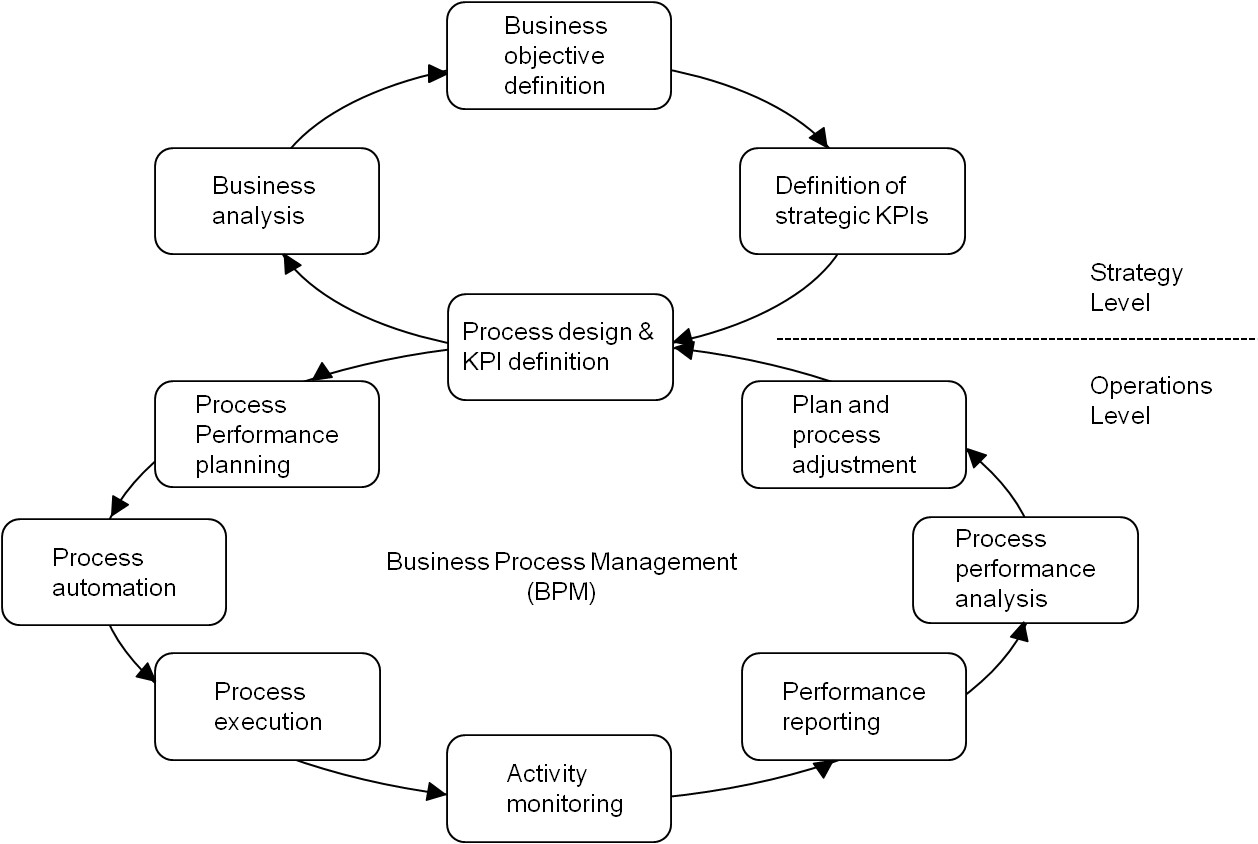
\includegraphics[width=0.8\linewidth]{Figures/Chapter5/Monitoring/Approach-Performance-Mgmt.jpg}
	\caption[Closed-loop Approach to Performance Management]{Closed-loop Approach to Performance Management \cite{book:AnalytInfSys}}
	\label{fig:Approach-Performance}
\end{figure}



\subsection{Architecture }

A Business Activity Monitoring (BAM) environment supported by Complex Event Processing consists of several elements necessary at build time and at runtime (see figure \ref{fig:BAMArchitecture}) and \cite{book:processmonitoring}, \cite{book:CEPinAction} , \cite{article:BlueprintEventBPM}). At build time a modeling environment should provide tools for designing processes (e.g. Metasonic Build) and defining process performance indicators (PPIs), BAM events, rules, thresholds etc. as well as parameters for their visualization in report and on dashboards. At runtime there are (1) event producers like a process engine (e.g. Metasonic Flow) or an ERP system (e.g. SAP) which feed events into an event cloud or stream (chronologically ordered). (2) Event Processing Agents (EPA) form the event processing logic. They process events based on metrics, event patterns, rules and other parameters specified at design time. Their basic logical functions include filtering and transforming events and detecting patterns among them. Global state elements allow them accessing data from outside the application (e.g. from an ERP system). EPAs put the results of their processing (also to be understood as events) out to Event Consumers (3) like dashboards or process engines. Input and Output Adapters (IA, OA) transform event data between different formats of system elements as necessary. All system elements involved form an Event Processing Network (EPN), in which events are exchanged by communication mechanisms.

\begin{figure}[htbp]
	\centering
	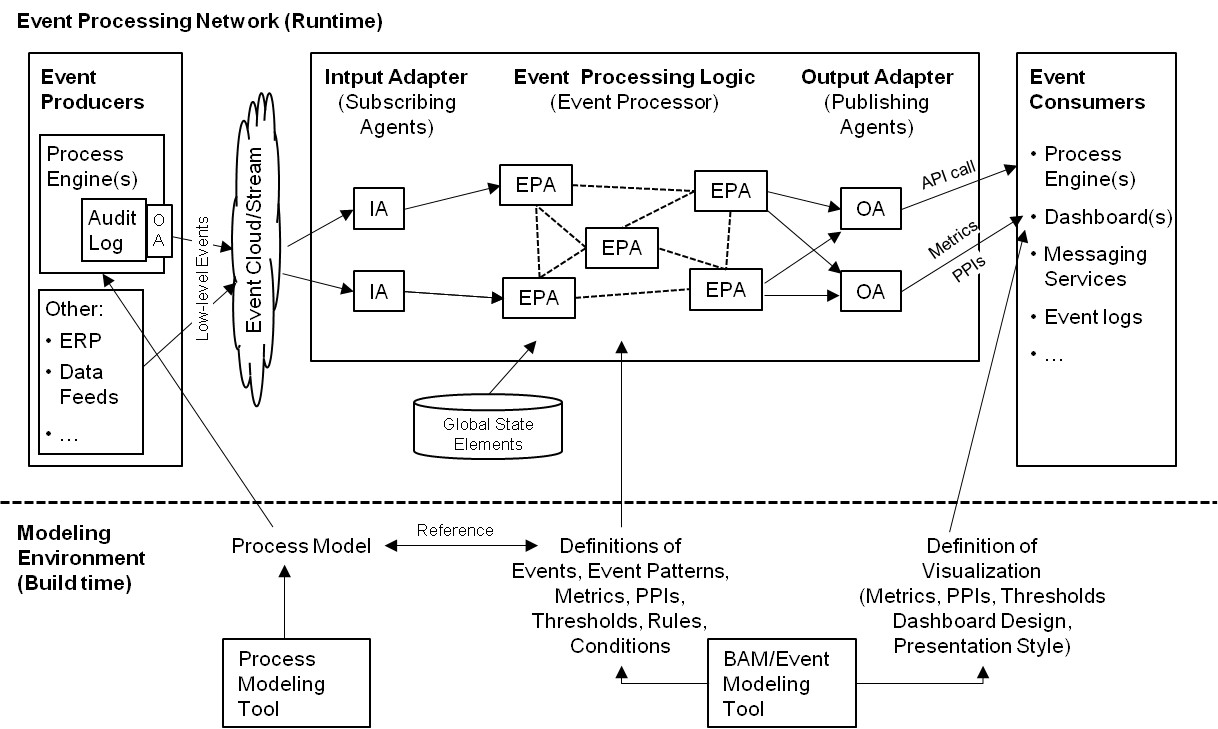
\includegraphics[width=0.9\linewidth]{Figures/Chapter5/Monitoring/Integrated-BAM-CEP-Architecture-27.jpg}
	\caption[Integrated BAM/CEP Architecture 27]{Integrated BAM/CEP Architecture \cite{book:processmonitoring}}
	\label{fig:BAMArchitecture}
\end{figure}



\subsection{Modeling BAM Parameters at Build Time}

As mentioned in the last section it is necessary not only to model the processes, but also numerous pieces of information relevant for a sound process monitoring in the sense of Business Activity Monitoring (BAM model). These can be derived from answers to questions like what, when, how and how often should be measured by whom \cite{book:ProzesseSchmelzer}. The information should also include how single metrics are to be aggregated in order to determine Process Performance Indicators (PPIs). For systematically collecting and documenting the necessary information fact sheets or templates for metrics and performance indicators have been developed \cite{book:KennzahlenIT}, \cite{book:ITControlling}. Figure \ref{tbl:Fact-Sheet}  shows an extract of a sample fact sheet defined for the average processing time of activities (see also \cite{article:SBPMCosting}, \cite{book:MonitoringSubjekt} ).


\begin{table}[htbp]
	\footnotesize
	\centering
	\begin{tabular}[t]{@{}l p{0.5\linewidth} p{0.3\linewidth} @{}}
		\toprule
		\textbf{Attribute} & \textbf{Content} \\
		\midrule
		\\
		 & \textbf{Characteristics}
		\\
		Identifier & Average activity time
		\\
		Description & Average time of a process activity within a certain period
		\\
		To-be value/unit & tbd specifically (min.)
		\\
		Tolerance range/unit & tbd specifically (\%)
		\\
		Escalation Rules/ Actions & In case of violation alert the process owner and start escalation process (tbd specifically)
		\\
		Addressees & Process Owner, Middle Mangement, Accountants (tbd specifically)
		Responsibility	Process Owner (tbd specifically)
		\\
		&  &
		\\
		& \textbf{Measuring and Computing}
		\\
		Measuring Object & All instances of the process 'Purchase Order'
		\\
		(Single) Metrics & Start time and end time of all activities of the process
		\\
		Measuring Method & Read time stamps for beginning and end of activities written by Metasonic Flow
		\\
		Measuring Frequency & For every single instance as it occurs
		\\
		Algorithms & For computing period: Sum of processing time of all activities divided by number of instances

		\\
		Data Sources (general) & Tables in the database of Metasonic Suite:
		RT\_PROCDESC, RT\_PROCINST, REC\_PARADESC, REC\_RECTRANS, UM\_USER
		\\
		Data Sources (specific) & Activity processing time (for one instance):\newline
		\textbf{SELECT} TIMESTAMP1  \newline
		(\textbf{SELECT} STARTTIME \newline
		\textbf{FROM} RT\_PROCINST \newline
		\textbf{WHERE} RT\_PROCDESC = \textit{process (purchase order)}\newline
		\textbf{AND} ID = \textit{instance (9)}\newline
		\textbf{FROM} REC\_RECTRANS\newline
		\textbf{WHERE} RT\_STDESC = \textit{\textit{state (fill\_in\_form)}}\newline
		\textbf{AND} RT\_PROCINST = \textit{instance (9)}
		Completed instances: see separate fact sheet .
		\\
		Computing Period (time, no. of inst.) & Daily
		\\
		& \textbf{Presentation}
		\\
		Presentation Style & As-is value and to-be value in combination with a spark line showing the historical development, deviation from to-be value in \%
		\\
		Presentation Frequency & Weekly and in case of escalation
		\\
		Archiving & Stored in additional database table, linked with RT\_PROCDESC
		\\

\bottomrule
\end{tabular}
\caption{Fact Sheet for a PPI (extract)}
\label{tbl:Fact-Sheet}
\end{table}

Replacing the content column by more formal ontology-based linguistic patterns as suggested by Del-Rio-Ortega et al. (see table \ref{tbl:Fact-Sheet-PPI}) could help relating PPIs to elements of the process model, performing automated analysis \cite{article:ProcessPerfInd} and implementing the measurement at runtime.

\begin{table}[htbp]
	\footnotesize
	\centering
%	\begin{tabular}[t]{@{}1 p{0.3\linewidth} p{0.3\linewidth} p{0.4\linewidth} @{}}
	\begin{tabular}[t]{ p{2 cm} p{5 cm} p{5 cm} }	
	\toprule
		\textbf{Attribute} & \textbf{Linguistic Pattern}  & \textbf{Example}
		\\
		\midrule
		PPI-<ID> & <PPI descriptive name> & PPI-001 Average time of RFC analysis
		\\
		\midrule
		Process	& <process ID the PPI is related to> & Request for change (RFC)
		\\
		\midrule
		Goals & <strategic or operational goals the PPI is related to> & BG-002: Improve customer satisfaction \newline
		BG-014: Reduce RFC time to response
		\\
		\midrule
		Definition & The PPI is defined as \newline \{<DurationMeasure> \newline \textbar <CountMeasure> \newline \textbar <ConditionMeasure> \newline \textbar <DataMeasure> \newline \textbar <DerivedMeasure> \newline \textbar <AggregatedMeasure> \} \newline {[}expressed in <unit of measure>{]} &  The PPI is defined as the average of Duration of Analyse RFC activity
		\\
		\midrule
		Target & The PPI value must \newline \{be \{greater \textbar lower\} than \newline {[}or equal to{]} <bound> \newline \textbar be between <lower bound> and \newline <upper bound> {[}inclusive{]} \textbar \newline fulfil the following constraint: <target constraint>\} \} & The PPI value must be slower than or equal to 1 working day
		\\
		\midrule
		Scope & The process instances considered for this PPI are \newline \{the last <n> ones \textbar those in the analysis period <AP-x> \} & The process instances considered for this PPI are the last 100 ones
		\\
		\midrule
		Source & <source from which the PPI measure can be obtained> &	Event logs of BPMS
		\\
		\midrule
		Responsible & \{ <role> \textbar <department> \textbar <organization> \textbar <person> \} &	Planning and quality manager
		\\
		\midrule
		Informed & \{ <role> \textbar <department> \textbar <organization> \textbar <person> \} & CIO
		\\
		\midrule
		Comments & <additional comments about the PPI> & Most RFCs are created after 12:00
		\\
\bottomrule
\end{tabular}
\caption{PPI Template based on Linguistic Patterns \cite{article:ProcessPerfInd}}
\label{tbl:Fact-Sheet-PPI}
\end{table}





Friedenstab et al. argue that such linguistic patterns do not fit to the usually graphical modeling of processes which makes integration difficult \cite{article:BPMNActivityMon}. The authors discuss some more approaches to BAM modeling. With regard to the limitations revealed, they present a BAM-related extension of the graphical Business Process Model Notation (BPMN) \cite{article:BPMNActivityMon}.
Using an abstract language syntax based on the Unified Modeling Language (UML) they started defining meta models for language constructs needed for BAM as there are Duration, Frequency, Composed Basic Measure, Aggregated Measure, Filter, Target Definition, Actions, Measure-based Expressions and Dashboard. Figure \ref{fig:Meta-Model} depicts the example for the duration of elements on different levels of detail, where the grey colored parts indicate references to the BPMN specification.

\begin{figure}[htbp]
	\centering
	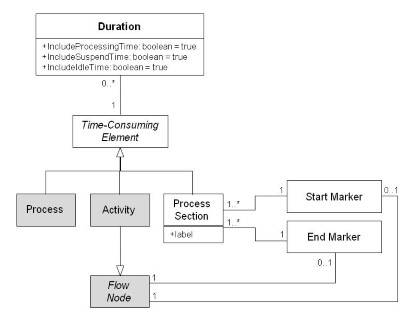
\includegraphics[width=0.9\linewidth]{Figures/Chapter5/Monitoring/Meta-Mode-fo-Duration-relate-to-BPMN-1.jpg}
	\caption[Meta Model for Duration (related to BPMN) 12]{Meta Model for Duration (related to BPMN) \cite{article:BPMNActivityMon}}
	\label{fig:Meta-Model}
\end{figure}


In a second step Friedenstab et al. developed a concrete syntax allowing for modeling the abstract language elements with graphical symbols and text labels. Parts of it are visible in figure \ref{fig:Model-Cycle-Times}. The example shows the BAM model for determining the cycle times of a purchase order process modeled in BPMN (lower part). The upmost part for example expresses the fact that the overall cycle time (Duration) for the last 50 instances (Filter) has to be determined and displayed on the dashboard (Dashboard). Monitoring the average of the overall cycle time for completed instances controls the modeled business logic of the process. If it is above 48 hours goods are delivered with an express shipping if the average cycle time is more than. Otherwise standard shipping is carried out. A deviation also leads to an alert sent to the process owner, while in any case the average is to be presented on the dashboard. The latter is also valid for the third time-related metric in the example, the partial cycle-time for the company-internal part of the process, which is set into relation with the overall cycle time.

\begin{figure}[htbp]
	\centering
	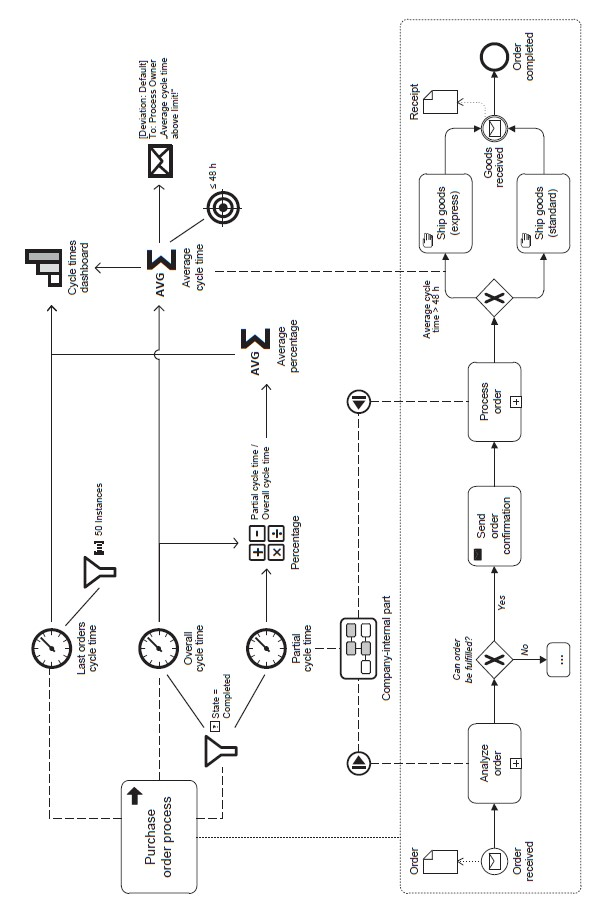
\includegraphics[width=0.9\linewidth]{Figures/Chapter5/Monitoring/BAM Model for Cycle Times.jpg}
	\caption[BAM Model for Cycle Times of a Purchase Order Process based on BPMN 12]{BAM Model for Cycle Times of a Purchase Order Process based on BPMN \cite{article:BPMNActivityMon}}
	\label{fig:Model-Cycle-Times}
\end{figure}


The concept presented by Friedenstab et al. is thoroughly thought-out and clearly and precisely elaborated. The idea now is to adapt it to Subject-oriented Business Process Management and relate the abstract syntax to the S-BPM meta model instead of BPMN. Due to S-BPM being a more precise and comprehensive notation than BPMN \cite{article:BPMNYAWLPatterns} the mapping should be possible without problems. Table \ref{tbl:MonBPMNSBPM} compares the BPMN specification elements used by \cite{article:BPMNActivityMon} with the ones appropriate in S-BPM \cite{Flei12}.


\begin{table}[htbp]
	\footnotesize
	\centering
	\begin{tabular}[t]{@{}l p{0.3\linewidth} p{0.4\linewidth} p{0.5\linewidth} @{}}
	\toprule
	\textbf{BAM Language Syntax Construct} & \textbf{Used BPMN Specification Element}  & \textbf{Suitable S-BPM Specification Element}\\
	\midrule\\
	Duration (Time-Consuming Element) &	Process, Activity, Flow Nodes&	Process, Subject Behaviour States (Function, Send, Receive, Start, End)
	\\
	Frequency
	(Countable Element)&	Process, Activity, Data Objects, Data States &	Process, Subject Behaviour States (Function, Send, Receive), Business Objects and their States
	\\
	Actions &	Process	 & Process
	\\
	Measure-based Expressions &	Expression, Sequence Flow &	Incoming Message
	\\
	\bottomrule
\end{tabular}
\caption{BPMN and S-BPM Specifications used in BAM Constructs}
\label{tbl:MonBPMNSBPM}
\end{table}

The remaining constructs as well as the extensions do not depend on the process modeling language and thus are not included in the table.
On the other hand S-BPM, following its paradigm of regarding subjects, predicates and objects as equally important parts of a process, offers the subject as an additional specification element to add . In figure \ref{fig:Meta-Model-S_BPM} we modified the picture of figure \ref{fig:Meta-Model} by replacing the BPMN by S-BPM elements and adding the subject. This allows modeling the determination of the overall time a subject (respectively the allocated resource(s)) spends on working on a process instance. This is of interest for cost-related analysis.

\begin{figure}[htbp]
	\centering
	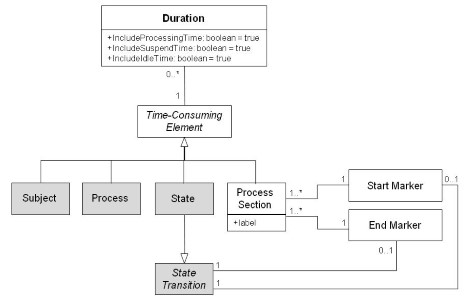
\includegraphics[width=0.9\linewidth]{Figures/Chapter5/Monitoring/Meta-Mode-fo-Duration-relate- to-SBPM.jpg}
	\caption[Meta Model for Duration (related to S-BPM)]{Meta Model for Duration (related to S-BPM)}
	\label{fig:Meta-Model-S_BPM}
\end{figure}


In order to show how the BAM language syntax constructs can be related to subject-oriented models we designed the purchase order process in S-BPM. Due to missing information in the BPM model some assumptions were necessary like who performs the process steps (subjects). We then added the BAM modeling symbols to create a monitoring model similar to that in figure \ref{fig:Meta-Model-S_BPM}.
The result is depicted in the following graph. In the lower part it includes the subject interaction diagram (SID) of the process. The SID shows the subjects involved and how they coordinate themselves in the course of action by exchanging messages. In the monitoring model in the upper part a difference can be seen. The partial cycle time for the company-internal activities can be modeled by just relating the clock symbol to the subject "Sales". In the example this subject represents all steps carried out within the organization. In the same way we can determine the cycle time for the other subjects.

\begin{figure}[htbp]
	\centering
	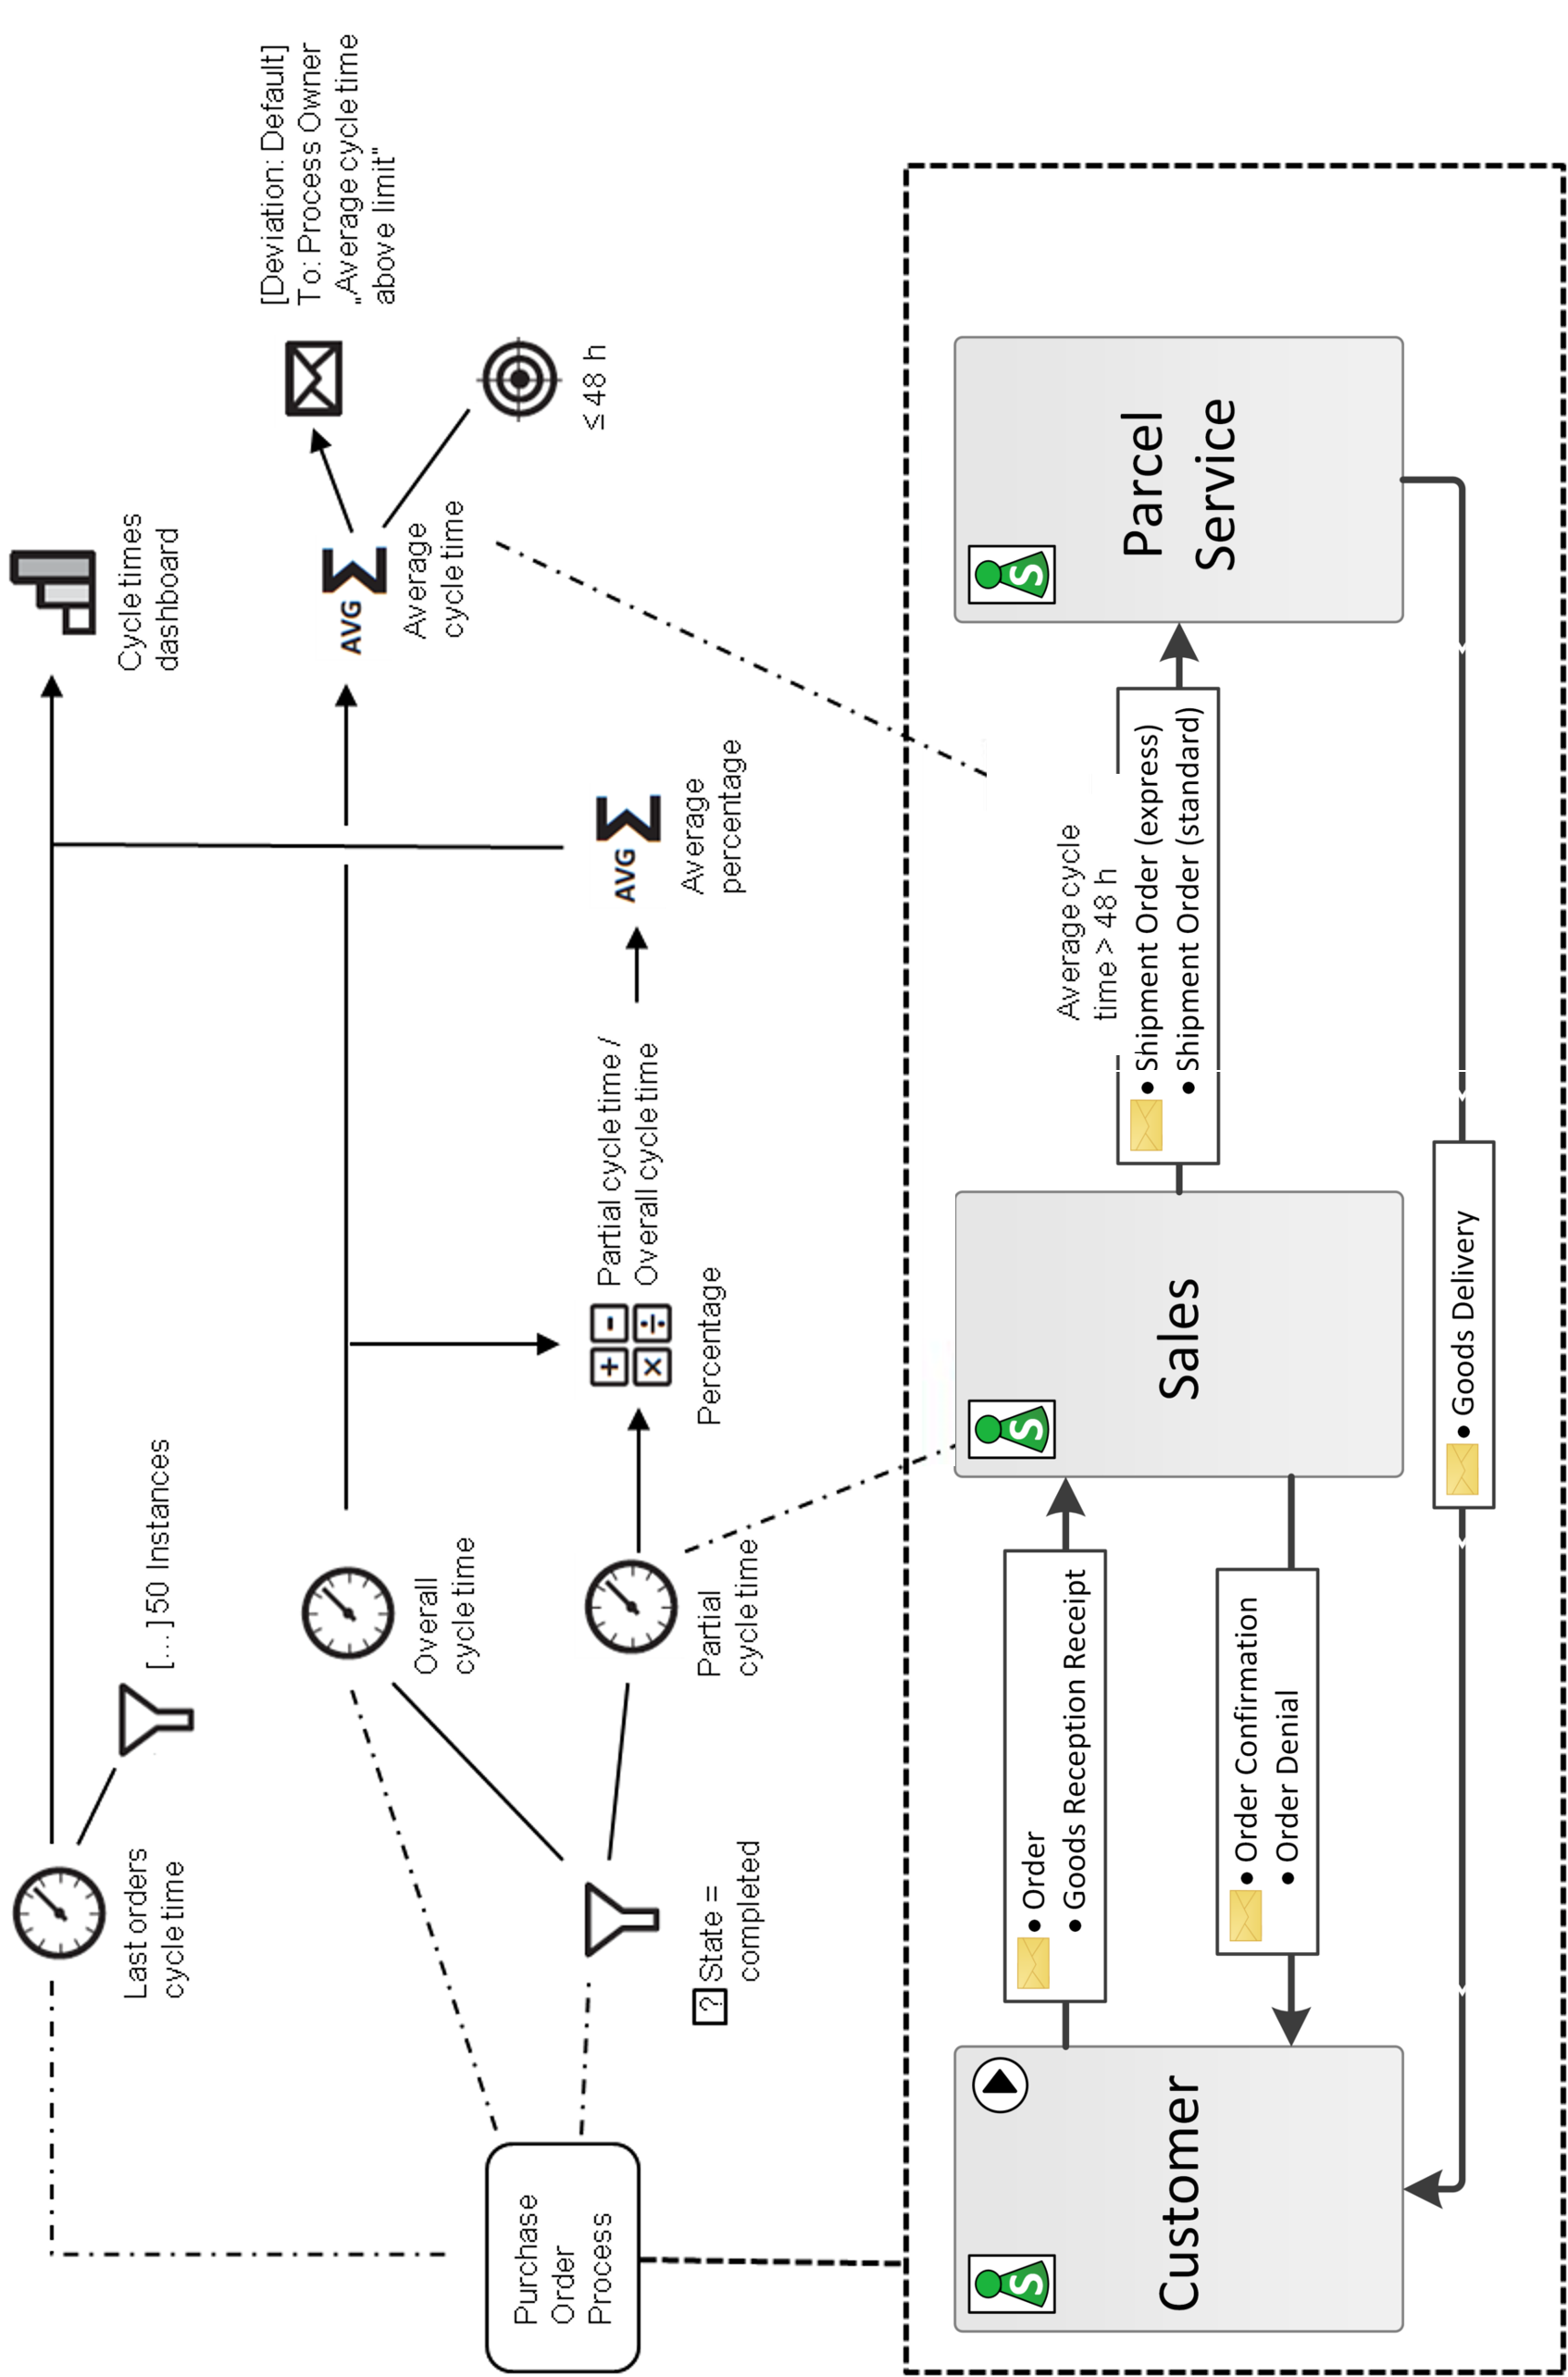
\includegraphics[width=0.9\linewidth]{Figures/Chapter5/Monitoring/BAM-Model-fo- Cycle-Times-of-a-Purchase-Order-Process-based-on-S-BPM_NEW.png}
	\caption[BAM Model for Cycle Times of a Purchase Order Process based on S-BPM]{BAM Model for Cycle Times of a Purchase Order Process based on S-BPM}
	\label{fig:Cycle-Time-SBPM}
\end{figure}

Given a special information demand a more granular modeling of BAM parameters is possible on the subject behavior level. Figure \ref{fig:BAM-Cycle-Time} for example details the behavior of "Sales" including all receive, send and functional states walked through by the subject. The symbols indicate that the average cycle time between order reception and confirming the order to the customer should be measured. In the same way cycle times between states in behaviours of different subjects can be modelled.


\begin{figure}[htbp]
	\centering
	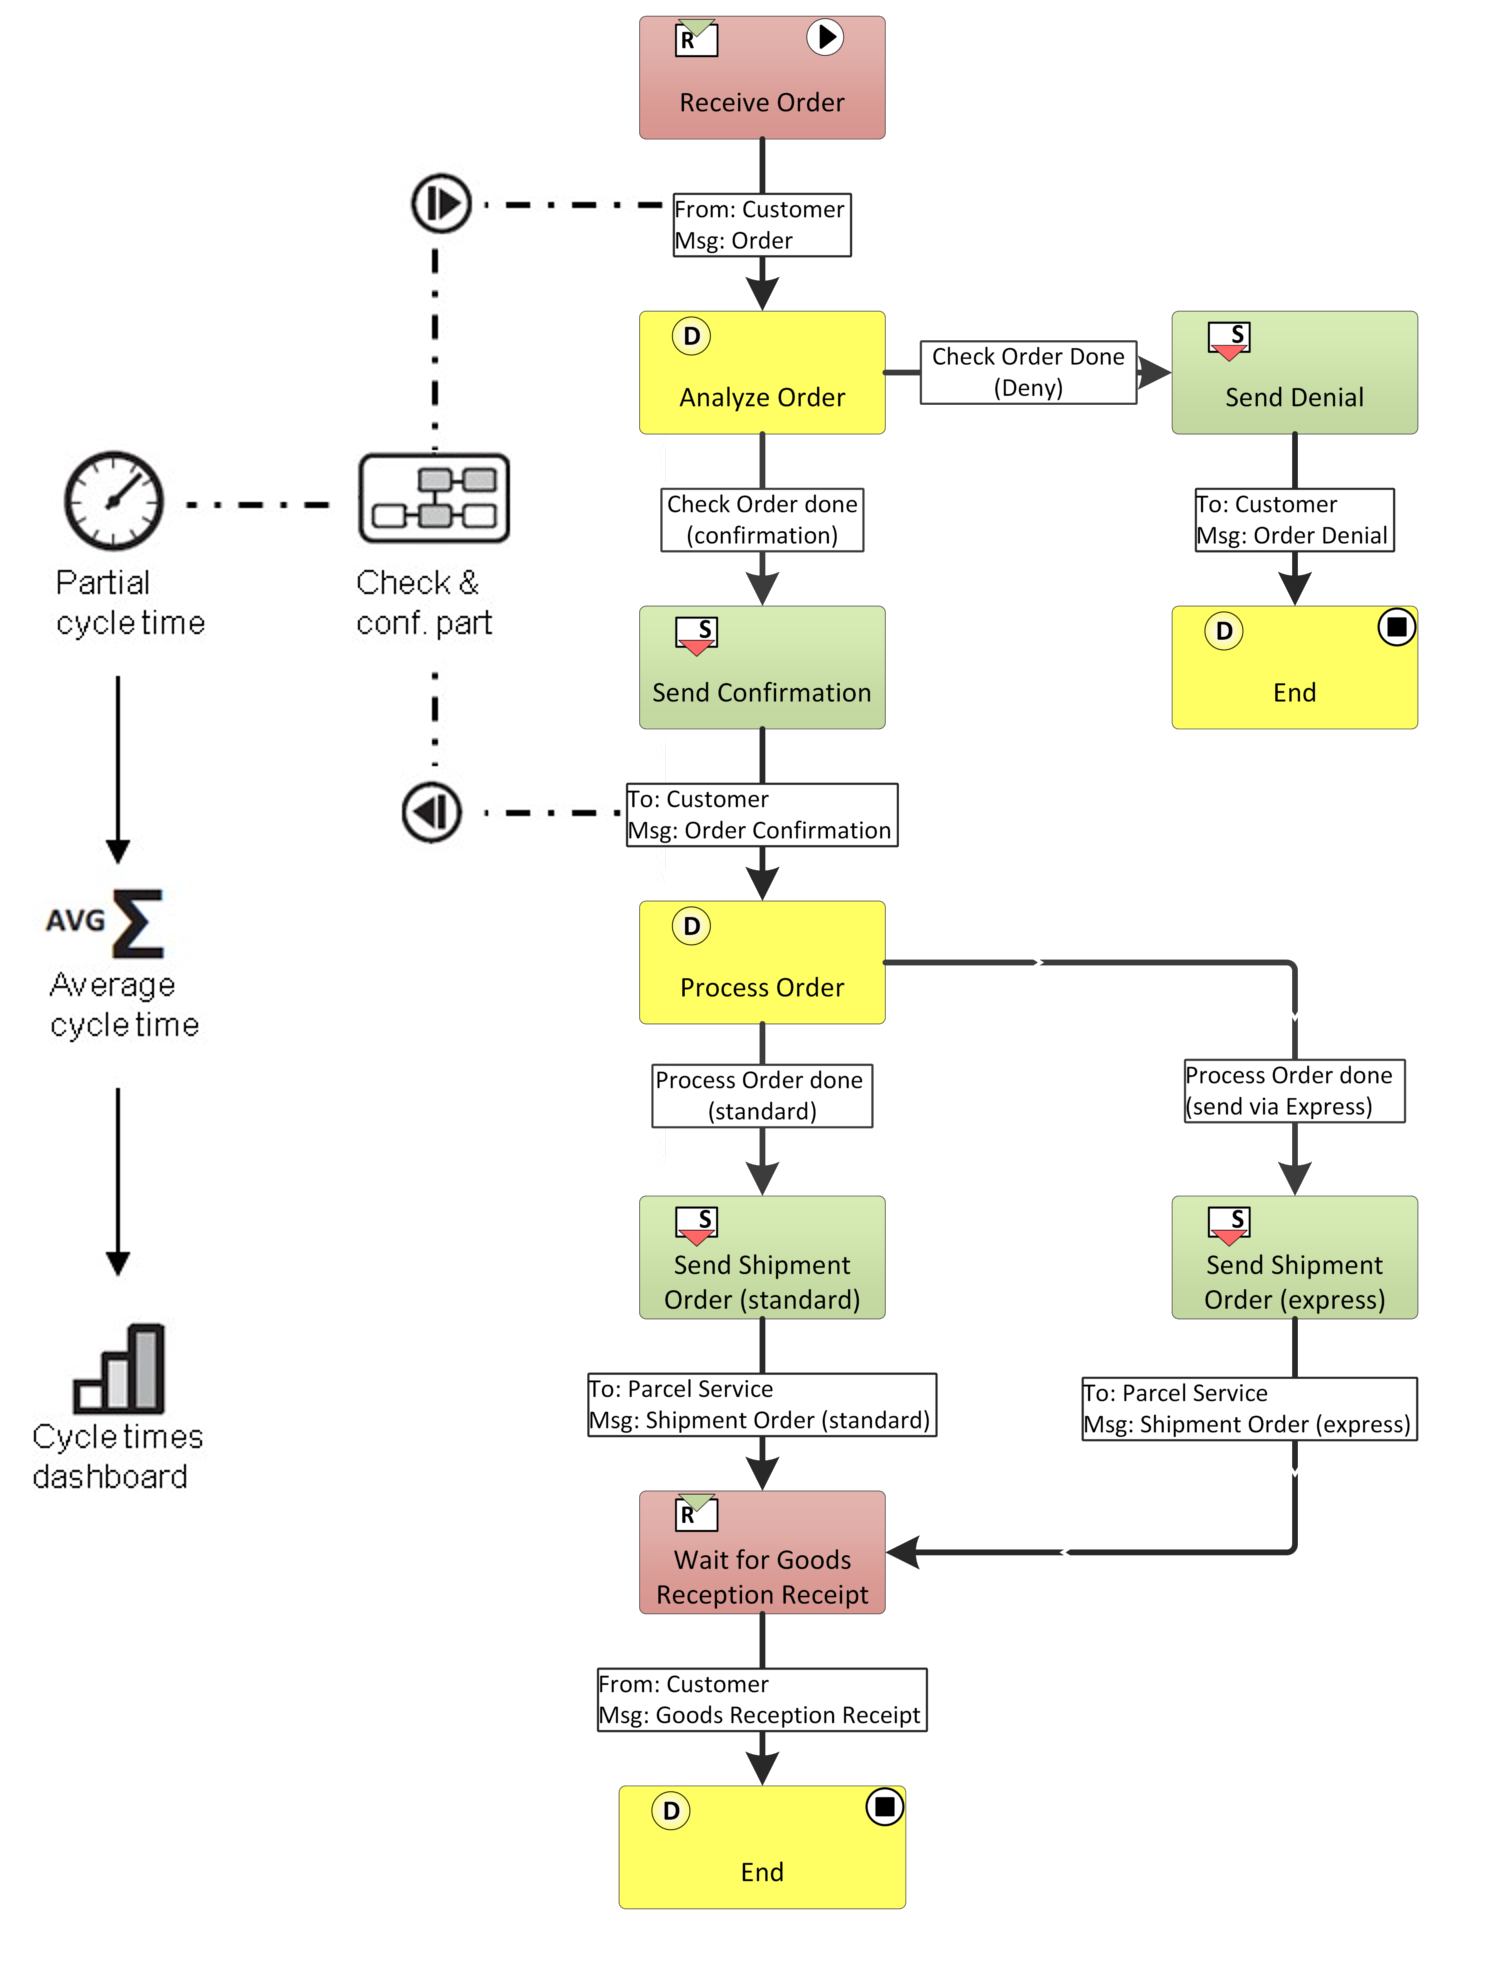
\includegraphics[width=0.9\linewidth]{Figures/Chapter5/Monitoring/BAM-Model-for-Cycle-Time-of-a-Process-Section-based-on-S-BPM_NEW.png}
	\caption[BAM Model for Cycle Time of a Process Section based on S-BPM]{BAM Model for Cycle Time of a Process Section based on S-BPM}
	\label{fig:BAM-Cycle-Time}
\end{figure}

Back on the level of subject interaction diagram we could also model to determine the overall time for receiving (waiting), sending and doing, both by process and by subject. Modeling on the two diagram levels reduces complexity.

\subsection {Conclusion and future Work}
This contribution systematized Business Process Monitoring and shed some light on the current state of monitoring in the context of S-BPM. Starting there we emphasized Business Activity Monitoring and took a closer look to the modelling of BAM parameters. We showed that the approach for BPMN presented by Friedenstab et al. can be adapted to S-BPM with little effort and that S-BPM shows additional potential to further develop the concept.
\\
\subsection{Future Work}

Due to the novel conceptual integration addressed, several aspects and topics need to be addressed by future research:
\begin{list}{-}{spacing}
	\item Extension of the structural semantics in OWL with possibilities to add Process Performance Indicators
	\item ASM definition of execution semantics for throwing events if process performance indicator boundaries are violated.
	\item ASM definition of execution semantics for handling violation events
\end{list}